\documentclass{standalone}
\usepackage{tikz}
\usetikzlibrary{patterns, positioning}
\usepackage[sfdefault]{ClearSans} %% option 'sfdefault' activates Clear Sans as the default text font
\usepackage[T1]{fontenc}

\begin{document}
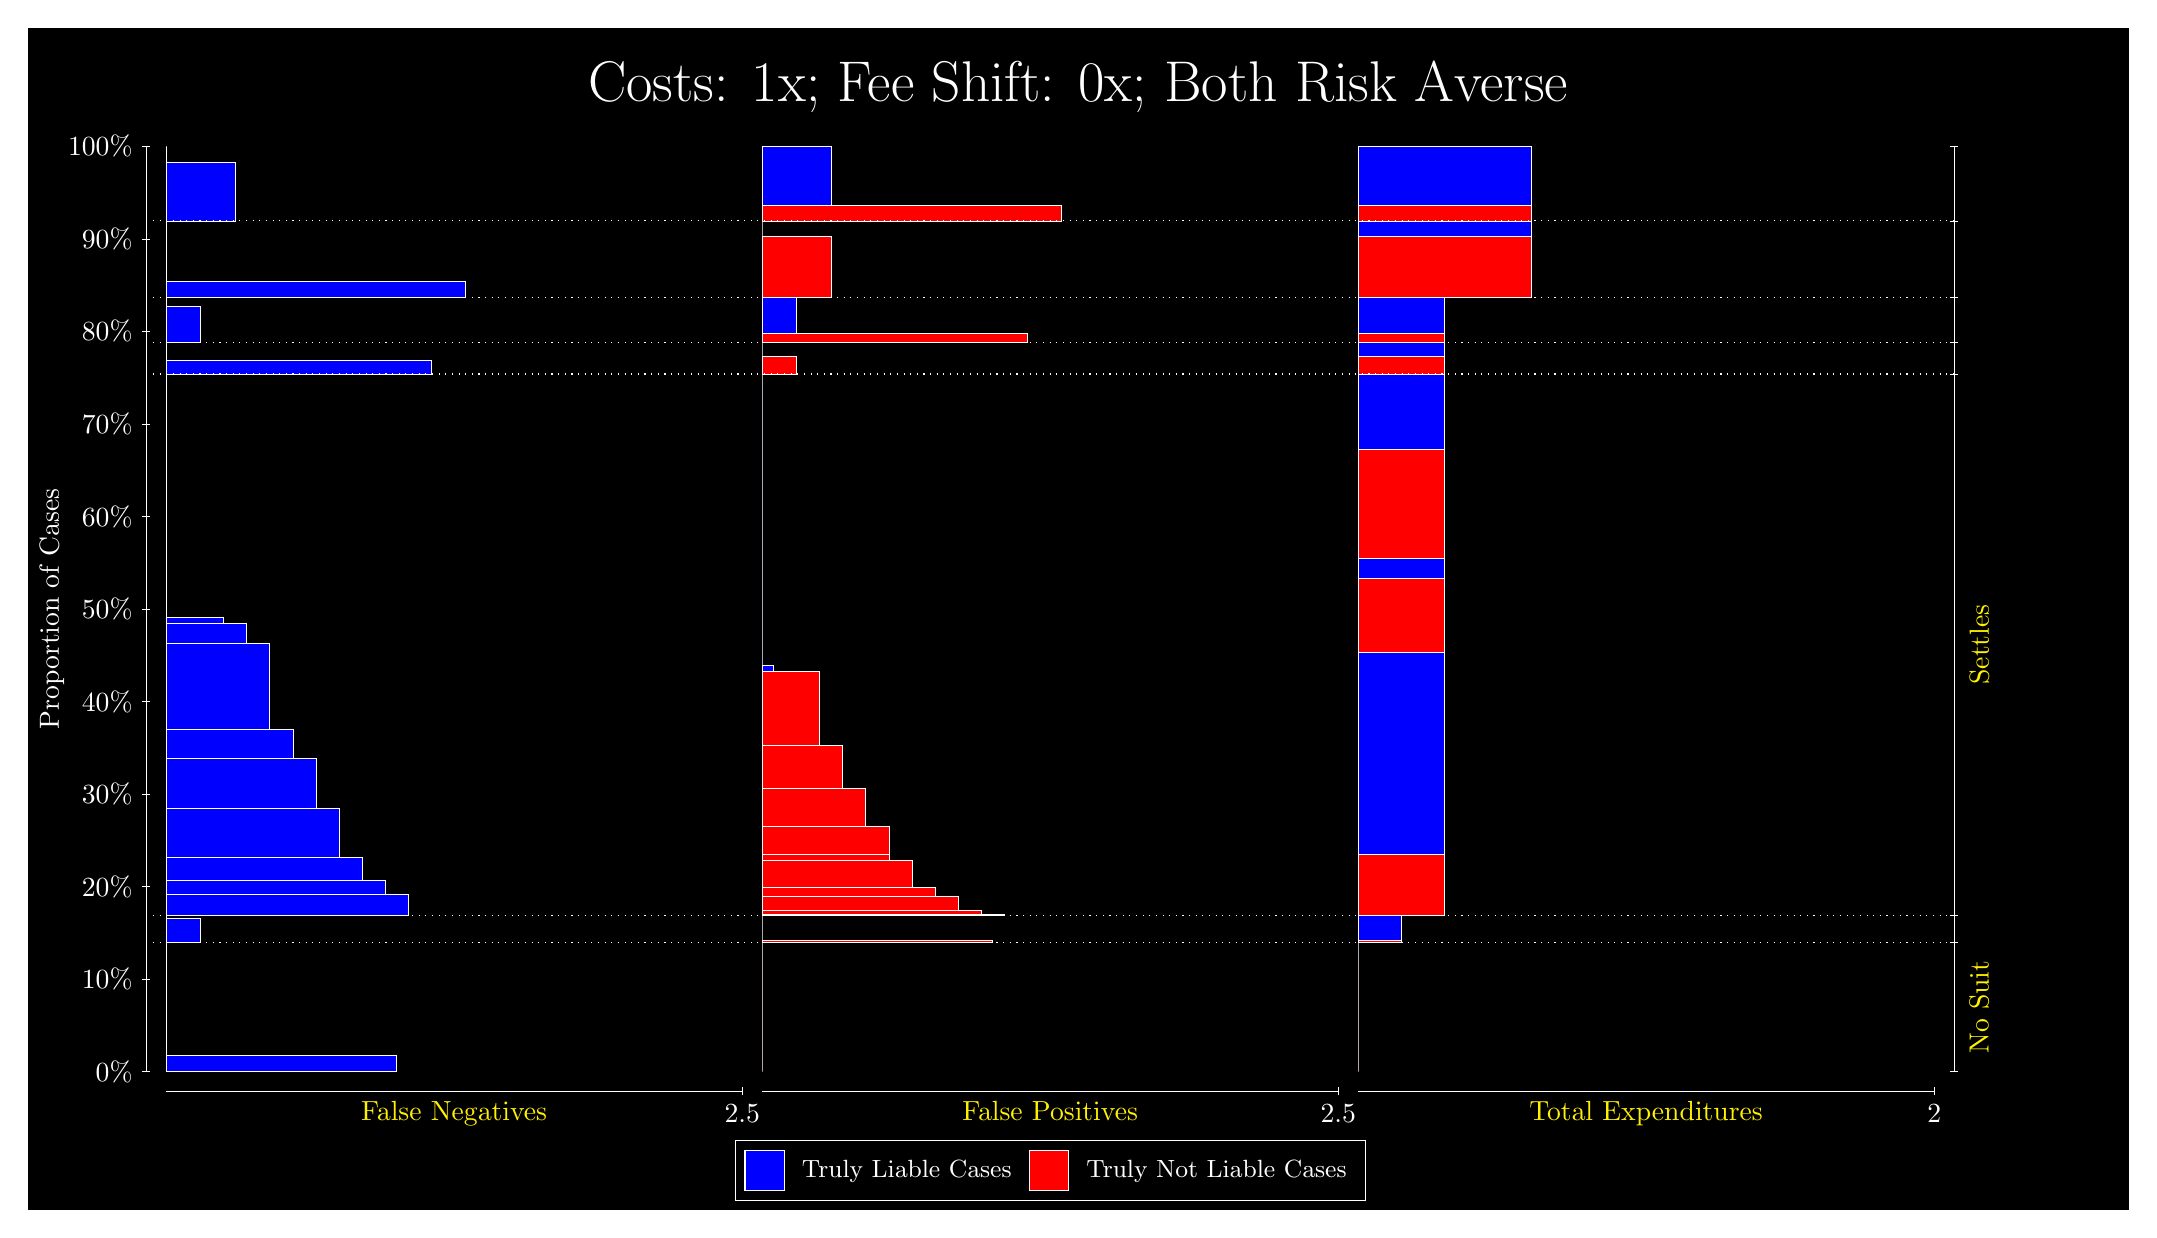
\begin{tikzpicture}
\draw[fill=black] (0,0) rectangle (26.667,15);
\draw[text=white] (0,13.5) rectangle (26.667,15) node[midway] {\huge Costs: 1x; Fee Shift: 0x; Both Risk Averse};
\draw[white, very thin] (1.5,1.75) -- (1.5,13.5);
\node[rotate=90, text=white, anchor=center] at (0.3, 7.625) {Proportion of Cases};
\draw[white, very thin] (1.45,1.75) -- (1.55,1.75);
\node[text=white, anchor=east] at (1.45, 1.75) {0\%};
\draw[white, very thin] (1.45,2.925) -- (1.55,2.925);
\node[text=white, anchor=east] at (1.45, 2.925) {10\%};
\draw[white, very thin] (1.45,4.1) -- (1.55,4.1);
\node[text=white, anchor=east] at (1.45, 4.1) {20\%};
\draw[white, very thin] (1.45,5.275) -- (1.55,5.275);
\node[text=white, anchor=east] at (1.45, 5.275) {30\%};
\draw[white, very thin] (1.45,6.45) -- (1.55,6.45);
\node[text=white, anchor=east] at (1.45, 6.45) {40\%};
\draw[white, very thin] (1.45,7.625) -- (1.55,7.625);
\node[text=white, anchor=east] at (1.45, 7.625) {50\%};
\draw[white, very thin] (1.45,8.8) -- (1.55,8.8);
\node[text=white, anchor=east] at (1.45, 8.8) {60\%};
\draw[white, very thin] (1.45,9.975) -- (1.55,9.975);
\node[text=white, anchor=east] at (1.45, 9.975) {70\%};
\draw[white, very thin] (1.45,11.15) -- (1.55,11.15);
\node[text=white, anchor=east] at (1.45, 11.15) {80\%};
\draw[white, very thin] (1.45,12.325) -- (1.55,12.325);
\node[text=white, anchor=east] at (1.45, 12.325) {90\%};
\draw[white, very thin] (1.45,13.5) -- (1.55,13.5);
\node[text=white, anchor=east] at (1.45, 13.5) {100\%};

\draw[white, very thin] (24.457,1.75) -- (24.457,13.5);
\draw[white, very thin] (24.407,1.75) -- (24.507,1.75);
\node[anchor=west] at (24.407, 1.75) {};
\draw[white, very thin] (24.407,3.3854) -- (24.507,3.3854);
\node[anchor=west] at (24.407, 3.3854) {};
\draw[white, very thin] (24.407,3.7367) -- (24.507,3.7367);
\node[anchor=west] at (24.407, 3.7367) {};
\draw[white, very thin] (24.407,10.608) -- (24.507,10.608);
\node[anchor=west] at (24.407, 10.608) {};
\draw[white, very thin] (24.407,11.011) -- (24.507,11.011);
\node[anchor=west] at (24.407, 11.011) {};
\draw[white, very thin] (24.407,11.584) -- (24.507,11.584);
\node[anchor=west] at (24.407, 11.584) {};
\draw[white, very thin] (24.407,12.553) -- (24.507,12.553);
\node[anchor=west] at (24.407, 12.553) {};
\draw[white, very thin] (24.407,13.5) -- (24.507,13.5);
\node[anchor=west] at (24.407, 13.5) {};

\draw[white, very thin, fill=blue] (1.75,1.75) rectangle (4.6775,1.9595);
\draw[white, very thin, fill=red] (1.75,1.9595) rectangle (1.75,3.3854);
\draw[white, very thin, fill=blue] (1.75,3.3854) rectangle (2.1891,3.7007);
\draw[white, very thin, fill=red] (1.75,3.7007) rectangle (1.75,3.7367);
\draw[white, very thin, fill=blue] (1.75,3.7367) rectangle (4.8239,3.9948);
\draw[white, very thin, fill=blue] (1.75,3.9948) rectangle (4.5312,4.178);
\draw[white, very thin, fill=blue] (1.75,4.178) rectangle (4.2384,4.4693);
\draw[white, very thin, fill=blue] (1.75,4.4693) rectangle (3.9457,5.0925);
\draw[white, very thin, fill=blue] (1.75,5.0925) rectangle (3.6529,5.7319);
\draw[white, very thin, fill=blue] (1.75,5.7319) rectangle (3.3602,6.1026);
\draw[white, very thin, fill=blue] (1.75,6.1026) rectangle (3.0674,7.1845);
\draw[white, very thin, fill=blue] (1.75,7.1845) rectangle (2.7746,7.4378);
\draw[white, very thin, fill=blue] (1.75,7.4378) rectangle (2.4819,7.5127);
\draw[white, very thin, fill=red] (1.75,7.5127) rectangle (1.75,10.608);
\draw[white, very thin, fill=blue] (1.75,10.608) rectangle (5.1167,10.781);
\draw[white, very thin, fill=red] (1.75,10.781) rectangle (1.75,11.011);
\draw[white, very thin, fill=blue] (1.75,11.011) rectangle (2.1891,11.465);
\draw[white, very thin, fill=red] (1.75,11.465) rectangle (1.75,11.584);
\draw[white, very thin, fill=blue] (1.75,11.584) rectangle (5.5558,11.783);
\draw[white, very thin, fill=red] (1.75,11.783) rectangle (1.75,12.553);
\draw[white, very thin, fill=blue] (1.75,12.553) rectangle (2.6283,13.301);
\draw[white, very thin, fill=red] (1.75,13.301) rectangle (1.75,13.5);
\draw[white, very thin, fill=red] (9.3189,1.75) rectangle (9.3189,3.176);
\draw[white, very thin, fill=blue] (9.3189,3.176) rectangle (9.3189,3.3854);
\draw[white, very thin, fill=red] (9.3189,3.3854) rectangle (12.246,3.4214);
\draw[white, very thin, fill=blue] (9.3189,3.4214) rectangle (9.3189,3.7367);
\draw[white, very thin, fill=red] (9.3189,3.7367) rectangle (12.393,3.7523);
\draw[white, very thin, fill=red] (9.3189,3.7523) rectangle (12.1,3.7946);
\draw[white, very thin, fill=red] (9.3189,3.7946) rectangle (11.807,3.9708);
\draw[white, very thin, fill=red] (9.3189,3.9708) rectangle (11.515,4.085);
\draw[white, very thin, fill=red] (9.3189,4.085) rectangle (11.222,4.4389);
\draw[white, very thin, fill=red] (9.3189,4.4389) rectangle (10.929,4.5118);
\draw[white, very thin, fill=red] (9.3189,4.5118) rectangle (10.929,4.8664);
\draw[white, very thin, fill=red] (9.3189,4.8664) rectangle (10.636,5.3483);
\draw[white, very thin, fill=red] (9.3189,5.3483) rectangle (10.344,5.8908);
\draw[white, very thin, fill=red] (9.3189,5.8908) rectangle (10.051,6.832);
\draw[white, very thin, fill=blue] (9.3189,6.832) rectangle (9.4652,6.9069);
\draw[white, very thin, fill=blue] (9.3189,6.9069) rectangle (9.3189,10.608);
\draw[white, very thin, fill=red] (9.3189,10.608) rectangle (9.758,10.838);
\draw[white, very thin, fill=blue] (9.3189,10.838) rectangle (9.3189,11.011);
\draw[white, very thin, fill=red] (9.3189,11.011) rectangle (12.686,11.13);
\draw[white, very thin, fill=blue] (9.3189,11.13) rectangle (9.758,11.584);
\draw[white, very thin, fill=red] (9.3189,11.584) rectangle (10.197,12.353);
\draw[white, very thin, fill=blue] (9.3189,12.353) rectangle (9.3189,12.553);
\draw[white, very thin, fill=red] (9.3189,12.553) rectangle (13.125,12.752);
\draw[white, very thin, fill=blue] (9.3189,12.752) rectangle (10.197,13.5);
\draw[white, very thin, fill=red] (16.888,1.75) rectangle (16.888,3.176);
\draw[white, very thin, fill=blue] (16.888,3.176) rectangle (16.888,3.3854);
\draw[white, very thin, fill=red] (16.888,3.3854) rectangle (17.437,3.4214);
\draw[white, very thin, fill=blue] (16.888,3.4214) rectangle (17.437,3.7367);
\draw[white, very thin, fill=red] (16.888,3.7367) rectangle (17.986,4.5118);
\draw[white, very thin, fill=blue] (16.888,4.5118) rectangle (17.986,7.0692);
\draw[white, very thin, fill=red] (16.888,7.0692) rectangle (17.986,8.0104);
\draw[white, very thin, fill=blue] (16.888,8.0104) rectangle (17.986,8.2685);
\draw[white, very thin, fill=red] (16.888,8.2685) rectangle (17.986,9.6474);
\draw[white, very thin, fill=blue] (16.888,9.6474) rectangle (17.986,10.608);
\draw[white, very thin, fill=red] (16.888,10.608) rectangle (17.986,10.838);
\draw[white, very thin, fill=blue] (16.888,10.838) rectangle (17.986,11.011);
\draw[white, very thin, fill=red] (16.888,11.011) rectangle (17.986,11.13);
\draw[white, very thin, fill=blue] (16.888,11.13) rectangle (17.986,11.584);
\draw[white, very thin, fill=red] (16.888,11.584) rectangle (19.083,12.353);
\draw[white, very thin, fill=blue] (16.888,12.353) rectangle (19.083,12.553);
\draw[white, very thin, fill=red] (16.888,12.553) rectangle (19.083,12.752);
\draw[white, very thin, fill=blue] (16.888,12.752) rectangle (19.083,13.5);
\draw[white, dotted] (1.5,3.3854) -- (24.457,3.3854);
\draw[white, dotted] (1.5,3.7367) -- (24.457,3.7367);
\draw[white, dotted] (1.5,10.608) -- (24.457,10.608);
\draw[white, dotted] (1.5,11.011) -- (24.457,11.011);
\draw[white, dotted] (1.5,11.584) -- (24.457,11.584);
\draw[white, dotted] (1.5,12.553) -- (24.457,12.553);
\draw[white, very thin] (1.75,1.5) -- (9.0689,1.5);
\node[text=yellow, anchor=north] at (5.4094, 1.5) {False Negatives};
\draw[white, very thin] (9.0689,1.45) -- (9.0689,1.55);
\node[text=white, anchor=north] at (9.0689, 1.45) {2.5};

\draw[white, very thin] (9.3189,1.5) -- (16.638,1.5);
\node[text=yellow, anchor=north] at (12.978, 1.5) {False Positives};
\draw[white, very thin] (16.638,1.45) -- (16.638,1.55);
\node[text=white, anchor=north] at (16.638, 1.45) {2.5};

\draw[white, very thin] (16.888,1.5) -- (24.207,1.5);
\node[text=yellow, anchor=north] at (20.547, 1.5) {Total Expenditures};
\draw[white, very thin] (24.207,1.45) -- (24.207,1.55);
\node[text=white, anchor=north] at (24.207, 1.45) {2};

\node[text=yellow, centered, rotate=90] at (24.777, 2.5677) {No Suit};

\node[text=yellow, centered, rotate=90] at (24.777, 7.1724) {Settles};





\draw (12.978300999999998,1.5) node[draw=none] (baseCoordinate) {};
\begin{scope}[align=center]
        \matrix[scale=0.5, draw=white, below=0.5cm of baseCoordinate, nodes={draw}, column sep=0.1cm]{
            \node[rectangle, draw, minimum width=0.5cm, minimum height=0.5cm, fill=blue] {}; &
            \node[draw=none, font=\small, text=white] (B) {Truly Liable Cases}; &
            \node[rectangle, draw, minimum width=0.5cm, minimum height=0.5cm, fill=red] {}; &
            \node[draw=none, font=\small, text=white] (B) {Truly Not Liable Cases}; \\
            };
\end{scope}

\end{tikzpicture}
\end{document}